\initial{T}ruth be told, water has already been found on Mars.
Both poles have ice caps containing solid water \cite{MARSwater}.
Unfortunately, solid water does not have the same solvating and lubricating properties as liquid water. Therefore it will not support molecular processes essential for life.
However, dry channels and craters probably formed by erosion suggest that liquid water (or some other liquid) was once present on Mars.

\begin{center}
	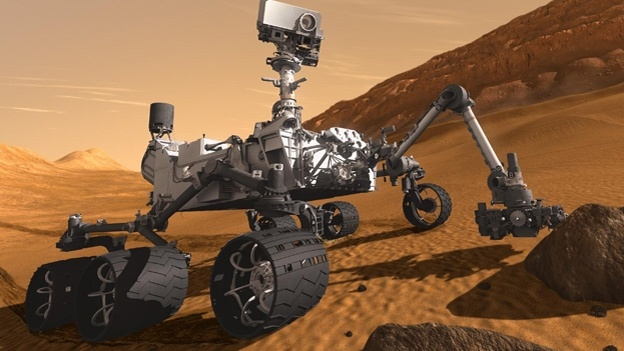
\includegraphics[width=0.45\textwidth]{Curiosity.jpg}
	NASAs Mars rover.
\end{center}

The best signs of life in space are therefore the discoveries of molecules we know can only be formed in contact with water.
For example, in 2002, Mars 2001 Odyssey, which is orbitting Mars, found the spectral signature of hematite, a molecule formed in water.
This mineral was later discovered by Opportunity, one of the two twin rovers exploring Mars from 2004 to 2010.
Furthermore, in 2005, Spirit, the other twin, found high concentrations of carbonate which originates in wet, near-neutral conditions. 
Carbonate actually dissolves in acid, which means that the water on this area could not have been acidic.
Hematite and carbonate are not the only minerals Curiosity is treasure hunting for.
In general, the rover uses its incredible instruments to study many different properties of the Martian surface.